\documentclass{article}

%packages
\usepackage{hyperref}
\usepackage[ngerman]{babel}
\usepackage[utf8]{inputenc}
\usepackage[left=2cm,right=2cm]{geometry}
\usepackage{arial}
\usepackage{graphicx}
\usepackage{eurosym}
\usepackage{amsmath}
\usepackage[backend=biber]{biblatex}

%farben setup für links
\hypersetup{
    colorlinks=true,
    linkcolor=black,
    filecolor=magenta,      
    urlcolor=cyan,
}

%pfad für images
\graphicspath{{img/}}

%lade das literaturverzeichnis
\addbibresource{literatur.bib}


%beginn des dokuments
\begin{document}

%Deckblatt
\newpage
\begin{titlepage}
	\centering
	Dokumentation zur betrieblichen Projektarbeit
\end{titlepage}
\newpage


%Inhaltsverzeichnis
\newpage
\tableofcontents
\newpage

%Abbildungsverzeichnis
\newpage
\listoffigures
\newpage

%Beginn des Dokuments

\section{Einleitung}
Dieser Abschnitt führt in das Projekt ein.

\subsection{Projektumfeld}
- Kurze Vorstellung des Ausbildungsbetriebs (Geschäftsfeld, Mitarbeiterzahl usw.)

- Wer ist Auftraggeber/Kunde des Projekts?

\subsection{Projektziel}

\subsection{Projektbegründung}

\subsection{Projektschnittstellen}

\subsection{Projektabgrenzung}

\section{Analyse}

\subsection{IST-Analyse}

\subsection{Wirtschaftlichkeitsanalyse}
%Leerzeichen können mit dem Tilde Zeichen (~) gesetzt werden (Alt Gr + tilde auf tastatur)
\[ \frac{100~Euro}{200~Tage} \]

\section{Planung}

%Entwurfsphase
\section{Entwurf}

\subsection{Benutzeroberfläche}

\subsubsection{Mitarbeiterbereich}

\subsubsection{Admin Bereich}

\subsection{Datenmodell}
%mit datenmodell abbildung

\subsection{Geschäftslogik}
%darstellung der Logik des Moduls als Programmaublaufplan/Komponenten/Sequenzdiagramm

%Implementierungsphase
\section{Implementierung}
\subsection{Implementierung der Datenstrukturen}
\subsection{Implementierung der Benutzeroberfläche}
% z.b. benutzeroberfläche mit html und css entwickelt
\subsection{Implementierung der Geschäftslogik}

%
\section{Validierungsphase}
%welche tests wurden durchgeführt (unit tests/ whitebox/ blackbox)

\section{Einführungsphase}
%wie lief das deployment ab (manuell/ automatisch mit pipelines)
%migration von altdaten (z.b. aus alter Zeiterfassung)
%schulungen für mitarbeiter durchgeführt?


\section{Dokumentation}
%wie wurde dokumentiert (php doc)
%anwenderdokumentation (d.h. für alle mitarbeiter, nicht nur IT leute)

\section{Fazit}
\subsection{Soll-/Ist-Vergleich}
\subsection{Gelerntes?}
\subsection{Ausblick}
%weiterentwicklung des projektes in der Zukunft


\section{Anhang}

\subsection{Abbildungsverzeichnis}

\subsubsection{Nutzwertanalyse}
\begin{center}
	\centering
	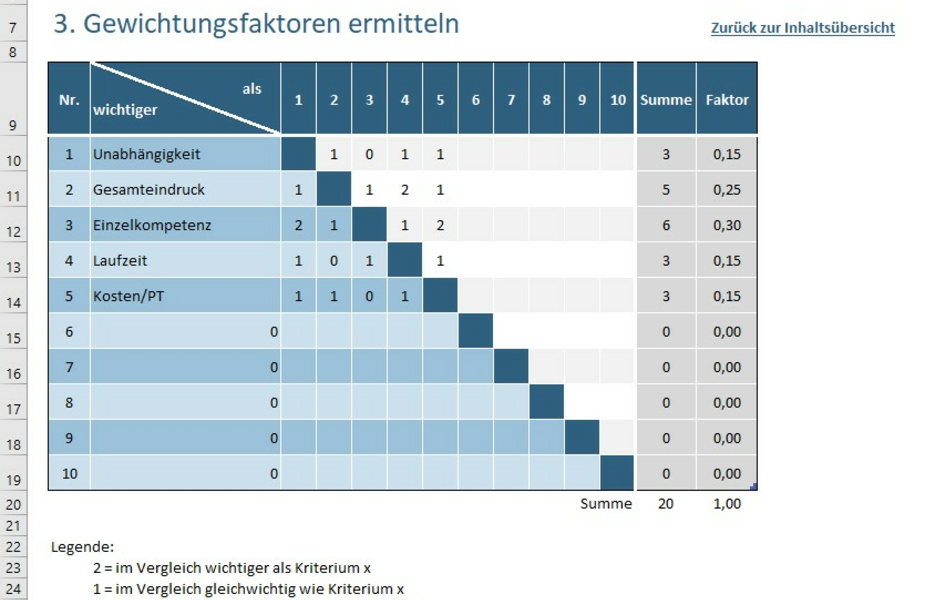
\includegraphics[scale=0.2]{nutz}
	\label{fig:nutz}
\end{center}


\subsection{Literaturverzeichnis}
Die mathematischen Beispiele stammen aus \autocite{Graham1995}.

Weitere Verweise: \parencite{Graham1995} oder \textcite{Thomas2008} oder sogar
\citetitle{Graham1995}.

\autocite[56]{Thomas2008}

\autocite[Siehe][45-48]{Graham1995}

Gemeinsam \autocite{Graham1995,Thomas2008}

\printbibliography

\end{document}


